\documentclass{standalone}
\usepackage{tikz}
\usepackage{ctex,siunitx}
\setCJKmainfont{Noto Serif CJK SC}
\usepackage{tkz-euclide}
\usepackage{amsmath}
\usetikzlibrary{patterns, calc}
\usetikzlibrary {decorations.pathmorphing,decorations.pathreplacing,decorations.shapes,}
\begin{document}
\small
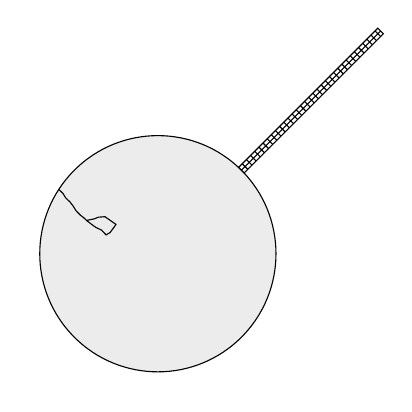
\begin{tikzpicture}[>=latex,scale=1.0]
  % \useasboundingbox(-1.0,-1.4)rectangle(3.5,3.7);
  \begin{scope}[rotate=45]
    \draw[fill=lightgray!30](0,0)circle(1.5);
    \draw[pattern=crosshatch](1.5,-0.05)rectangle(4,0.05);
    \draw[thin,decorate,decoration={random steps, segment length =2pt,amplitude=0.5pt}](102:1.5)--(110:1.0)--(115:0.7)--(100:0.65)--(100:0.82)--(110:1.0);
  \end{scope}
\end{tikzpicture}
\end{document}